\documentclass[aspectratio=169]{beamer}
\usepackage[utf8]{inputenc}
\usepackage{hyperref}
\usepackage{amsmath,amsfonts,amsthm,bm}
\usepackage{color}
\usepackage{graphicx} % Allows including images
\usepackage{subcaption}
\usepackage{booktabs} % Allows the use of \toprule, \midrule and \bottomrule in tables
\usepackage{tikz}
\usetikzlibrary{automata,positioning}
%\usepackage{pgfplots}
\usepackage{adjustbox}
\usepackage{listings}
\usepackage{courier}
\usepackage[version=4]{mhchem}
\usepackage{array}
\usepackage{modiagram}

\lstset{ %
  basicstyle=\scriptsize\ttfamily, % fonts that are used for the code
  breakatwhitespace=false,         % sets if automatic breaks should only happen at whitespace
  %breaklines=true,                 % sets automatic line breaking
  %captionpos=b,                    % sets the caption-position to bottom
  commentstyle=\color{gray}\textit,    % comment style
  keepspaces=true,                 % keeps spaces in text, useful for keeping indentation of code (possibly needs columns=flexible)
  keywordstyle=\color{blue},       % keyword style
  language=Python,                 % the language of the code
  %otherkeywords={*,...},          % if you want to add more keywords to the set
  rulecolor=\color{black},         % if not set, the frame-color may be changed on line-breaks within not-black text (e.g. comments (green here))
  showspaces=false,                % show spaces everywhere adding particular underscores; it overrides 'showstringspaces'
  showstringspaces=false,          % underline spaces within strings only
  showtabs=false,                  % show tabs within strings adding particular underscores
  stringstyle=\color{red}, % string literal style
  tabsize=4,	                   % sets default tabsize to 2 spaces
  columns=fixed                    % Using fixed column width (for e.g. nice alignment)
}

\hypersetup{
    colorlinks=true,
    linkcolor=red,
    filecolor=magenta,      
    urlcolor=red,
}

\DeclareMathOperator*{\argmax}{argmax}
\DeclareMathOperator*{\argmin}{argmin}
\let \vec \mathbf

\newcommand{\classname}{NANO266}
\newcommand{\classyear}{Fall 2024}
\mode<presentation> {
    \usetheme{CambridgeUS}
    \setbeamertemplate{footline}[text line]{%
      \parbox{\linewidth}{\vspace*{-8pt}\classname\hfill\classyear\hfill\insertpagenumber}}

    %\setbeamertemplate{footline}[page number]
    \setbeamertemplate{navigation symbols}{}
}


\title[\classname Beyond the HF Approximation]{\classname~- Quantum Mechanical Modeling of Materials and Nanostructures\\Beyond the HF Approximation}

\author{Shyue Ping Ong}
\institute[UCSD]{University of California, San Diego\\
\medskip
}
\date{\classyear} % Date, can be changed to a custom date

\begin{document}


\begin{frame}
    \titlepage % Print the title page as the first slide
\end{frame}

\begin{frame}{Overview}
In this lecture, we will only touch on conceptual underpinnings of how correlation is included, without going too much into the details of the methods. Most of the advanced methods are far too computationally expensive and limited to small system sizes, which makes them less useful for the materials scientist at this time. It suffices that you understand them at a conceptual level, and if you are interested (or they become more accessible in future), there are many excellent works on the subject.


\begin{alertblock}{Definition of electron correlation}
\begin{equation*}
    E_{corr} = E_{exact} - E_{HF} 
\end{equation*}
\end{alertblock}

\end{frame}


\begin{frame}{How might one improve on HF?}
\begin{columns}
    \column{0.5\linewidth}
    
    HF utilizes a single determinant. An obvious extension is:
    \begin{equation*}
        \psi = c_0 \psi_{HF} + c_1 \psi_{1} + c_2\psi_{2} + ...
    \end{equation*}

Types of correlation
\begin{itemize}
    \item Dynamical correlation: From ignoring dynamic electron-electron interactions. $c_0$ is much larger than other coefficients.
    \item Non-dynamical correlation: Arises from single determinant nature of HF. Several $c_i$ with magnitude similar to $c_0$.
\end{itemize}
    \column{0.5\linewidth}
\begin{figure}
    \centering
    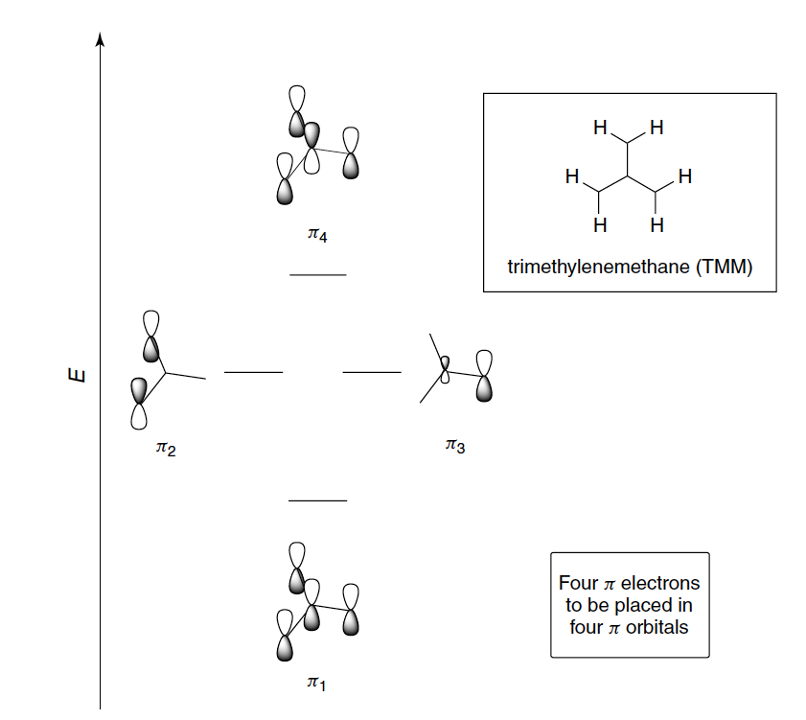
\includegraphics[width=0.7\linewidth]{lectures/figures/3_degenerate_orbitals.png}
    \caption{Degenerate frontier orbitals cannot be represented with single determinant.}
\end{figure}
\end{columns}

\end{frame}

\begin{frame}{Multiconfiguration SCF}
Optimize orbitals for a combination of configurations (orbital occupations).\newline
\newline
Configuration state function (CSF): molecular spin state and occupation number of orbitals.\newline
\newline
Active space: orbitals that are allowed to be partially occupied (based on chemistry of interest).\newline
\newline
Scaling

\begin{equation*}
    \mbox{No. of CSFs for $m$ electrons in $n$ orbitals} = \frac{n!(n+1)!}{(\frac{m}{2})!(\frac{m}{2}+1)!(n-\frac{m}{2})!(n-\frac{m}{2}+1)!}
\end{equation*}

CAS: Complete Active Space (CASSCF)

\end{frame}

\begin{frame}{Full Configuration Interaction (CI)}
CASSCF calculation of all orbitals and all electrons.\newline
\newline
Best possible calculation within limits of basis set.\newline
\newline
Full CI + Infinite Basis Set = Exact Solution to Schr\"odinger Equation\newline
\newline
For small systems, can be used to benchmark other methods.
    
\end{frame}


\begin{frame}{Limitation Excitations in CI}
\begin{columns}
    \column{0.5\linewidth}
\begin{figure}
    \centering
    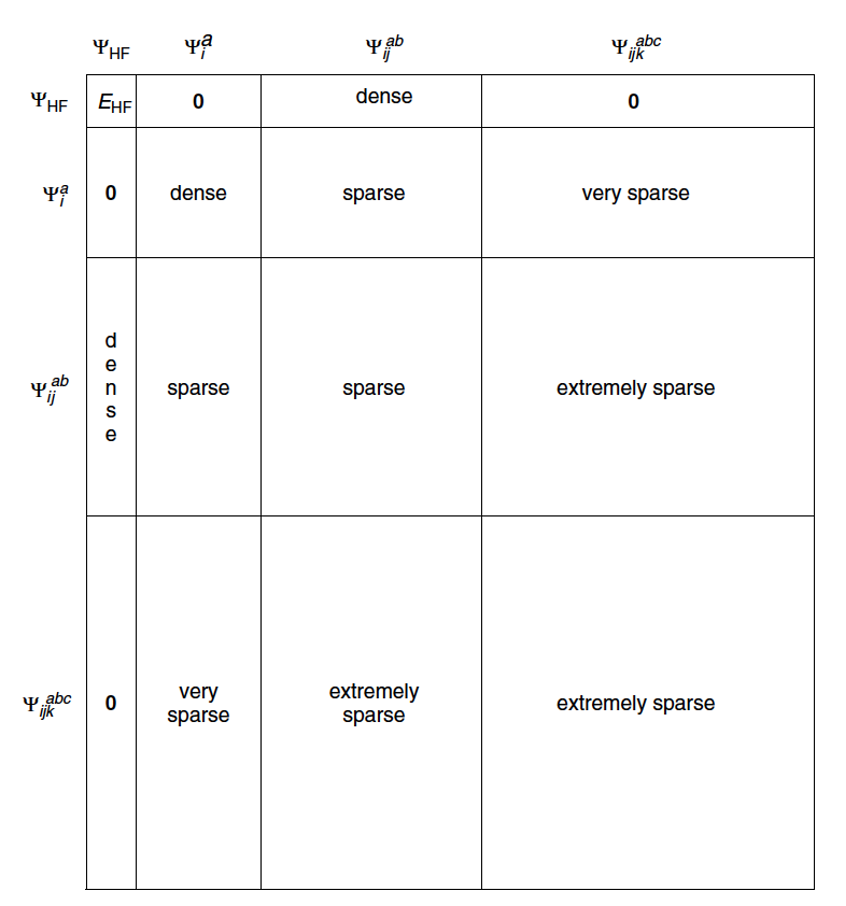
\includegraphics[width=0.8\linewidth]{lectures/figures/3_CI_excitations.png}
\end{figure}
    \column{0.5\linewidth}
CIS (CI singles)
\begin{itemize}
    \item Used for excited states.
    \item No use for ground states (single excitations do not mix with HF determinant).
\end{itemize}

CID (CI doubles)

CISD (CI singles doubles) - $N^6$ scaling

\end{columns}

\end{frame}


\begin{frame}{M{\o}ller-Plesset Perturbation Theory}
    Treats exact Hamiltonian as a perturbation on sum of one-electron Fock operators:
    \begin{equation*}
    \footnotesize
        H = H^{(0)}+ \lambda V = \sum_i f_i + \lambda V
    \end{equation*}
Expanding the ground state eigenfunctions and eigenvalues as a Taylor series in $\lambda$,
\begin{eqnarray*}
\footnotesize
\psi & = & \psi^{(0)} + \lambda \psi^{(1)} + \lambda^2 \psi^{(2)} + ..., \psi^{(k)} = \frac{1}{k!}\frac{\partial^k \psi}{\partial \lambda^k}\\
a & = & a^{(0)} + \lambda a^{(1)} + \lambda^2 a^{(2)} + ..., a^{(k)} = \frac{1}{k!}\frac{\partial^k a}{\partial \lambda^k}\\
H\psi & = & a\psi\\
(H^{(0)}+ \lambda V)\sum \lambda^k\psi^{(k)} & = & \sum \lambda^k a^{(k)}\sum \lambda^k\psi^{(k)}
\end{eqnarray*}
By equating powers of $\lambda$, we can derive $a^{(k)}$, the $k^{\mbox{th}}$ order corrections to $a^{(0)}$.
\end{frame}

\begin{frame}{MPn Methods}

\begin{columns}
    \column{0.5\textwidth}
MP1 = HF\newline
\newline
MP2
\begin{itemize}
    \item Second-order energy correction.
    \item Analytical gradients available.
    \item $N^5$ scaling.
\end{itemize}

MP(n $>$ 2)
\begin{itemize}
    \item No analytic gradients available.
    \item $> 95\%$ of electron correlation at $n=4$. 
\end{itemize}

    \column{0.5\textwidth}
Issues:
\begin{itemize}
    \item Perturbation theory works best when perturbation is small.
    \item In MPn, perturbation is full electron-electron repulsion!
    \item MPn is not variational! Possible for correlation to be larger than exact, but in practice, basis set limitations cause errors in the opposite direction.
\end{itemize}

\end{columns}

\end{frame}

\begin{frame}{Coupled Cluster}
    Full-CI wave function can be described as:
    \begin{equation*}
        \psi = e^{\vec{T}}\psi_{HF}
    \end{equation*}
    where $\vec{T}=\vec{T_1}+\vec{T_2}+\vec{T_3}+...$ is the cluster operator.


If we truncate at $\vec{T_2}$,expansion,
    \begin{equation*}
        \psi = [1+(\vec{T_1}+\vec{T_2})+\frac{(\vec{T_1}+\vec{T_2})^2}{2}+...]\psi_{HF}
    \end{equation*}

\begin{alertblock}{CCSD(T)}
\begin{itemize}
    \item Includes single/triples coupling term.
    \item Analytical gradients and second derivatives available.
    \item ``Gold standard'' in most quantum chemistry calculations.
\end{itemize}
\end{alertblock}

\end{frame}


\begin{frame}{Practical considerations}
\begin{columns}
    \column{0.4\textwidth}
Basis set convergence is a bigger problem for correlated calculations.\newline
\newline
Accuracy: HF $<$ MP2 $\sim$ MP3 $<$ CCD $<$ CISD $<$ QCISD $\sim$ CCSD $<$ MP4 $<$ QCISD(T) $\sim$ CCSD(T)\cite{foresmanExploringChemistryElectronic1996}
    \begin{figure}
        \centering
        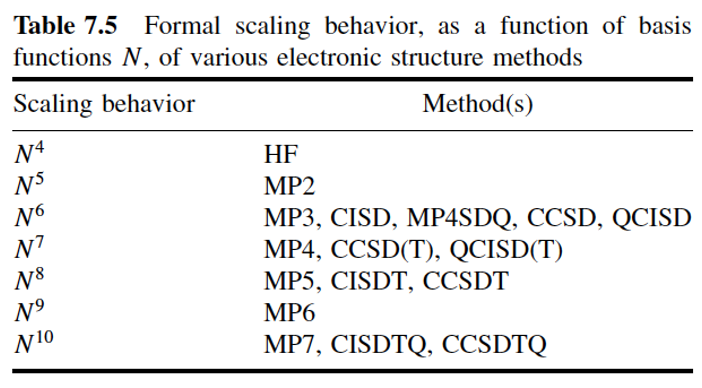
\includegraphics[width=0.9\linewidth]{lectures/figures/3_scaling.png}
    \end{figure}
\column{0.6\textwidth}
    \begin{figure}
        \centering
        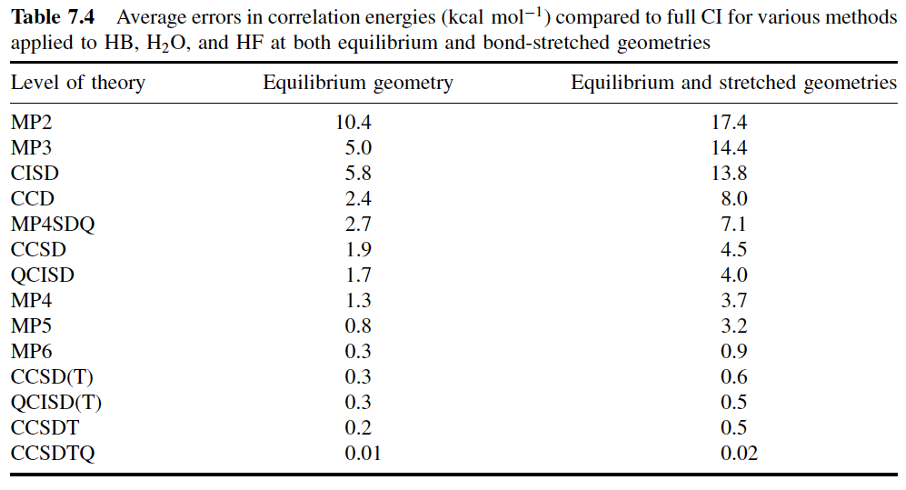
\includegraphics[width=\linewidth]{lectures/figures/3_correlation_energies_vs_FCI.png}
    \end{figure}
\end{columns}

\end{frame}


    \begin{frame}{Relative accuracy of variational methods}
\begin{figure}
    \centering
    \begin{subfigure}{0.45\textwidth}
    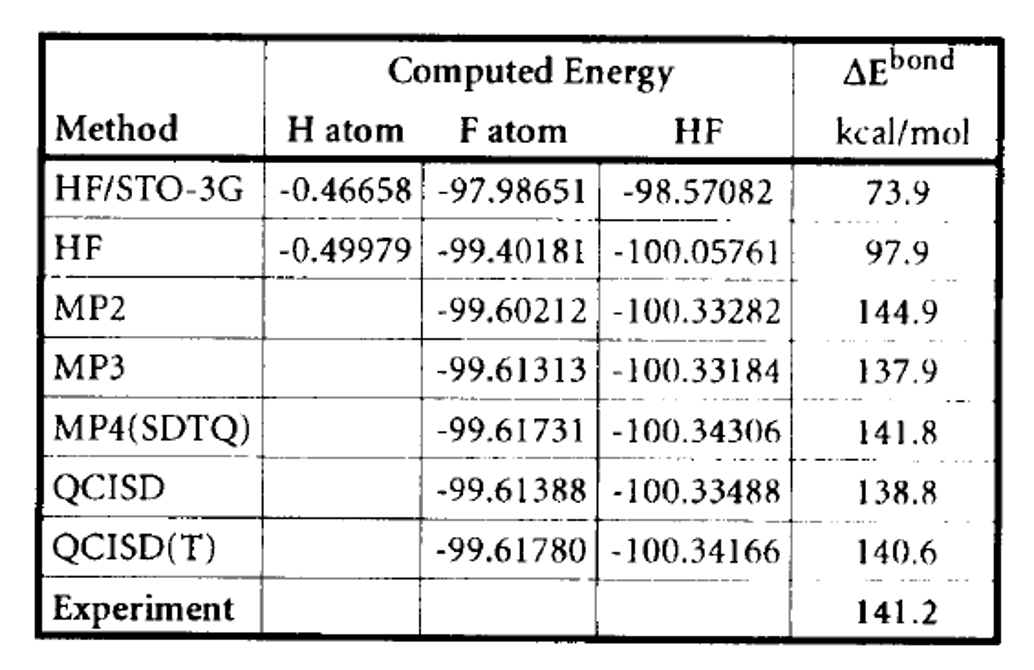
\includegraphics[width=\linewidth]{lectures/figures/3_dissociation_of_HF.png}
    \caption{Dissociation of HF.\cite{foresmanExploringChemistryElectronic1996}.}
    \end{subfigure}
    \begin{subfigure}{0.5\textwidth}
        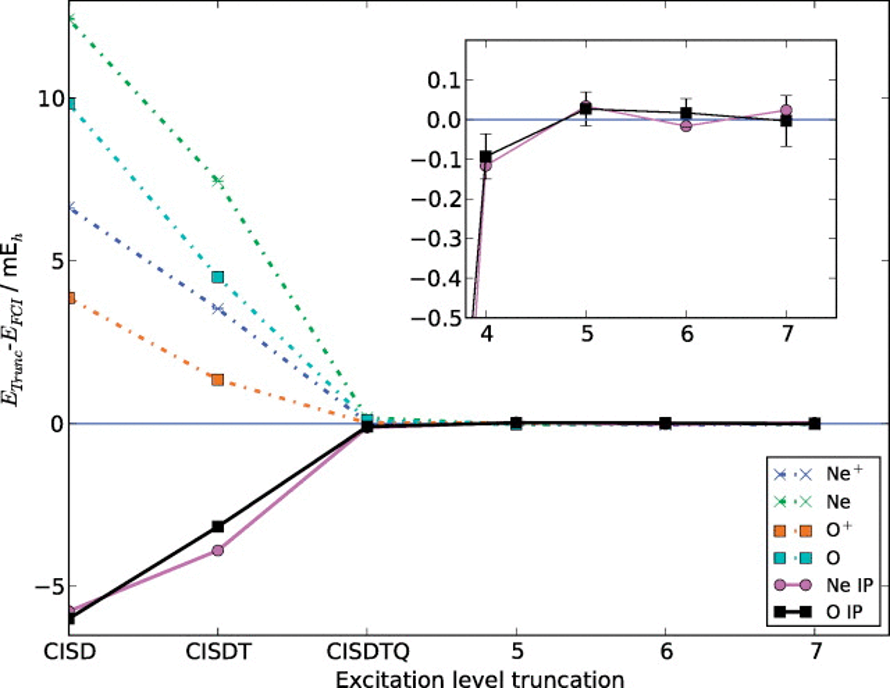
\includegraphics[width=0.8\linewidth]{lectures/figures/3_ionization_potentials.png}
    \caption{Ionization potentials of noble gases and ions. aug-cc-pVTZ basis set. Dashed lines: Difference in the total energy of each species compared to the FCI limit; Solid lines: Error in the IP.\cite{boothApproachingChemicalAccuracy2010}}
    \end{subfigure}
        
\end{figure}
        
    \end{frame}

\begin{frame}{Computational Cost}
    \begin{figure}
        \centering
        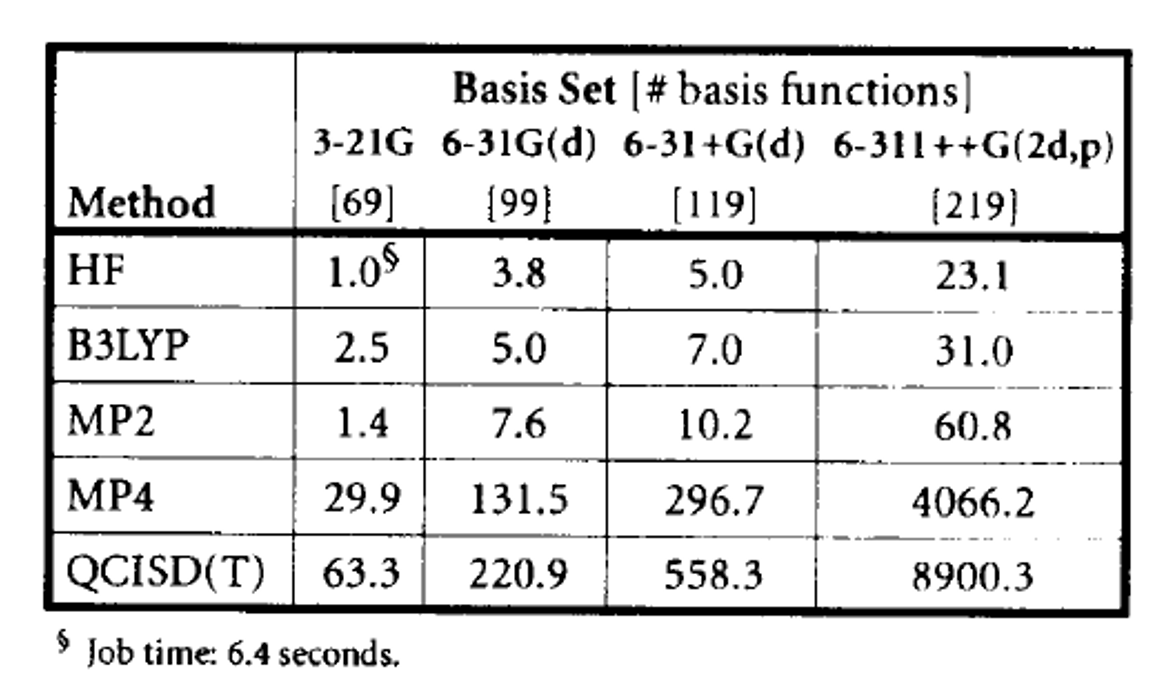
\includegraphics[width=0.65\linewidth]{lectures/figures/3_compute_cost.png}
        \caption{From \cite{foresmanExploringChemistryElectronic1996}.}
    \end{figure}
\end{frame}

\begin{frame}{Parametrized methods}
    \begin{figure}
        \centering
        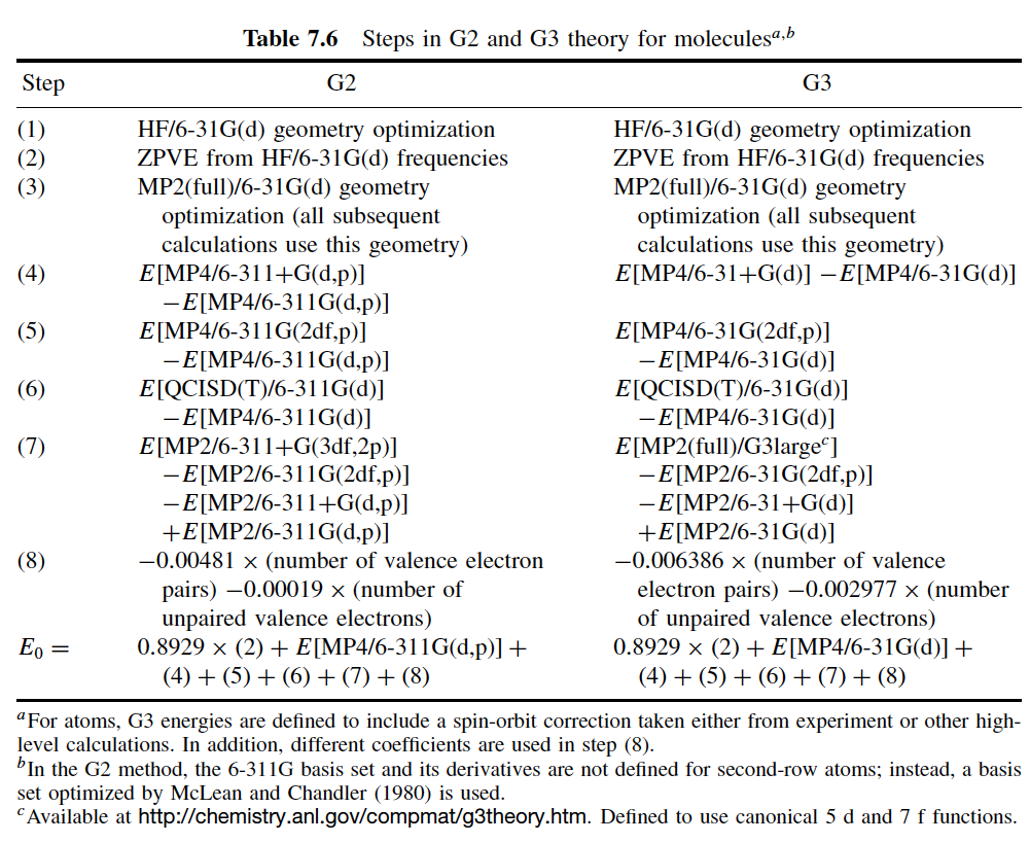
\includegraphics[width=0.5\linewidth]{lectures/figures/3_G2_G3.png}
        \caption{G2/G3 theory for accurate thermochemistry (errors $<$ 4 kcal / mol).}
    \end{figure}
\end{frame}

\begin{frame}[allowframebreaks]{Bibliography}
    \bibliographystyle{unsrt}
    \bibliography{refs}
\end{frame}



\begin{frame}
    \Huge{\centerline{The End}}
\end{frame}

\end{document}

